A point query is a database operation that finds the records that exactly match our query conditions. In this project, we perform point query on $1$-dimensional data and $2$ dimensional data. We assign the database records into pages, predict the page index with the index models and then perform sequential search on the predicted page. In order to evaluate the errors that different index models are making, we focus on predicting the page indices and ignore the sequential search operation on a specific page. 

\begin{mscexample}
For example, assume we have an $1$-dimensional array $[1,2,3,4]$ and two pages such that $[1,2]\in P_0$ and $[3,4]\in P_1$. A point query for $x=2$ is expected to return 0 as the page index.
\end{mscexample}

\subsubsection{Point Query with B-Tree}

B-tree and its variants have been widely used as indexes in databases. B-trees can be considered as a generalisation of binary search tree: In binary search tree, there is only one key and two children at most in the internal node. B-tree extends the nodes such that each node can contain several keys and children. The keys in a node serve as dividing points and separate the range of keys. With this structure, we make a multi-way decision based on comparisons with the keys stored at the node $x$.

In this section, we introduce the construction process of B-trees and then analyse its properties.

\subsubsection{Attributes and Properties}

Each node \texttt{x} in a B-tree has the following attributes:

\begin{itemize}
\item \texttt{x.n}: the number of keys currently stored in the node $x$.
\item \texttt{x.keys}: the stored keys of this node.
\item \texttt{x.leaf}: a bool value that determines if current node is a leaf node.
\item \texttt{x.children}: a list of its children. If \texttt{x} is a leaf node who has no children at all, then the list will be empty. We assume the children are \texttt{x.$c_1$,$\cdots$,x.$c_{x.n+1}$}, i.e. there will be $\texttt{x.n}+1$ children at most.
\end{itemize}

\noindent
With these attributes, a B-tree has the following properties:

\begin{itemize}
\item The number of children of a node is always $1$ bigger than the number of keys in a node.
\item Nodes in this tree have lower and upper bounds on the number of keys they can contain. These two bounds can be expressed in terms of a fixed integer $t$, which we call the \textbf{minimum degree} of this tree.
	\begin{enumerate}
		\item Each node, other than the root node, must contain at least $t-1$ keys. The root of the tree must have at least one key if the tree is not empty.
		\item Each node can contain at most $2t-1$ keys. A node is called \textbf{full} if it contains exactly $2t-1$ keys.
	\end{enumerate}
\item Inside each node, the keys are sorted in the non-decreasing order, so that we have \texttt{x.keys$_1\leq $} \texttt{x.keys$_2\leq \cdots \leq$} \texttt{x.keys$_{\texttt{x.n}}$}.
\item The keys \texttt{x.key$_i$} separate the ranges of keys stored in each subtree: if $k_i$ is any key stored in the subtree with a root \texttt{x.c$_i$}, then we have $k_1\leq$\texttt{x.keys$_1\leq $}$ k_2\leq$\texttt{x.keys$_2\leq $} $\cdots\leq$ \texttt{x.keys$_n\leq $}$k_{\texttt{x.n}+1}$.
\end{itemize}

In Fig. \ref{fig: B-tree}, we demonstrate an example B-tree whose minimum degree is $2$. In the following section, we will illustrate how to construct and insert keys into a B-tree.

\begin{figure}
\centering
B-tree and its variants have been widely used as indexes in databases. B-trees can be considered as a generalisation of binary search tree: In binary search tree, there is only one key and two children at most in the internal node. B-tree extends the nodes such that each node can contain several keys and children. The keys in a node serve as dividing points and separate the range of keys. With this structure, we make a multi-way decision based on comparisons with the keys stored at the node $x$.

In this section, we introduce the construction process of B-trees and then analyse its properties.

\subsubsection{Attributes and Properties}

Each node \texttt{x} in a B-tree has the following attributes:

\begin{itemize}
\item \texttt{x.n}: the number of keys currently stored in the node $x$.
\item \texttt{x.keys}: the stored keys of this node.
\item \texttt{x.leaf}: a bool value that determines if current node is a leaf node.
\item \texttt{x.children}: a list of its children. If \texttt{x} is a leaf node who has no children at all, then the list will be empty. We assume the children are \texttt{x.$c_1$,$\cdots$,x.$c_{x.n+1}$}, i.e. there will be $\texttt{x.n}+1$ children at most.
\end{itemize}

\noindent
With these attributes, a B-tree has the following properties:

\begin{itemize}
\item The number of children of a node is always $1$ bigger than the number of keys in a node.
\item Nodes in this tree have lower and upper bounds on the number of keys they can contain. These two bounds can be expressed in terms of a fixed integer $t$, which we call the \textbf{minimum degree} of this tree.
	\begin{enumerate}
		\item Each node, other than the root node, must contain at least $t-1$ keys. The root of the tree must have at least one key if the tree is not empty.
		\item Each node can contain at most $2t-1$ keys. A node is called \textbf{full} if it contains exactly $2t-1$ keys.
	\end{enumerate}
\item Inside each node, the keys are sorted in the non-decreasing order, so that we have \texttt{x.keys$_1\leq $} \texttt{x.keys$_2\leq \cdots \leq$} \texttt{x.keys$_{\texttt{x.n}}$}.
\item The keys \texttt{x.key$_i$} separate the ranges of keys stored in each subtree: if $k_i$ is any key stored in the subtree with a root \texttt{x.c$_i$}, then we have $k_1\leq$\texttt{x.keys$_1\leq $}$ k_2\leq$\texttt{x.keys$_2\leq $} $\cdots\leq$ \texttt{x.keys$_n\leq $}$k_{\texttt{x.n}+1}$.
\end{itemize}

In Fig. \ref{fig: B-tree}, we demonstrate an example B-tree whose minimum degree is $2$. In the following section, we will illustrate how to construct and insert keys into a B-tree.

\begin{figure}
\centering
B-tree and its variants have been widely used as indexes in databases. B-trees can be considered as a generalisation of binary search tree: In binary search tree, there is only one key and two children at most in the internal node. B-tree extends the nodes such that each node can contain several keys and children. The keys in a node serve as dividing points and separate the range of keys. With this structure, we make a multi-way decision based on comparisons with the keys stored at the node $x$.

In this section, we introduce the construction process of B-trees and then analyse its properties.

\subsubsection{Attributes and Properties}

Each node \texttt{x} in a B-tree has the following attributes:

\begin{itemize}
\item \texttt{x.n}: the number of keys currently stored in the node $x$.
\item \texttt{x.keys}: the stored keys of this node.
\item \texttt{x.leaf}: a bool value that determines if current node is a leaf node.
\item \texttt{x.children}: a list of its children. If \texttt{x} is a leaf node who has no children at all, then the list will be empty. We assume the children are \texttt{x.$c_1$,$\cdots$,x.$c_{x.n+1}$}, i.e. there will be $\texttt{x.n}+1$ children at most.
\end{itemize}

\noindent
With these attributes, a B-tree has the following properties:

\begin{itemize}
\item The number of children of a node is always $1$ bigger than the number of keys in a node.
\item Nodes in this tree have lower and upper bounds on the number of keys they can contain. These two bounds can be expressed in terms of a fixed integer $t$, which we call the \textbf{minimum degree} of this tree.
	\begin{enumerate}
		\item Each node, other than the root node, must contain at least $t-1$ keys. The root of the tree must have at least one key if the tree is not empty.
		\item Each node can contain at most $2t-1$ keys. A node is called \textbf{full} if it contains exactly $2t-1$ keys.
	\end{enumerate}
\item Inside each node, the keys are sorted in the non-decreasing order, so that we have \texttt{x.keys$_1\leq $} \texttt{x.keys$_2\leq \cdots \leq$} \texttt{x.keys$_{\texttt{x.n}}$}.
\item The keys \texttt{x.key$_i$} separate the ranges of keys stored in each subtree: if $k_i$ is any key stored in the subtree with a root \texttt{x.c$_i$}, then we have $k_1\leq$\texttt{x.keys$_1\leq $}$ k_2\leq$\texttt{x.keys$_2\leq $} $\cdots\leq$ \texttt{x.keys$_n\leq $}$k_{\texttt{x.n}+1}$.
\end{itemize}

In Fig. \ref{fig: B-tree}, we demonstrate an example B-tree whose minimum degree is $2$. In the following section, we will illustrate how to construct and insert keys into a B-tree.

\begin{figure}
\centering
\input{graphs/implementation/one-dim/b-tree}
\caption{An example of B-tree with the minimum degree $t=2$.}
\label{fig: B-tree}
\end{figure}

\subsubsection{Insertion in a B-tree}

With a B-tree, we cannot simply create a new leaf node and insert the new key as we do with a binary search tree, because the resulting tree will fail to be a valid B-tree. Instead, we need to insert the new key into an existing leaf node. If the node is not full, we can safely insert the new key. Otherwise, we will need to split the node around the median of its keys into two new nodes and promote the median key into its parent. In this process, we need to split the parent if its parent is also full.

In the insertion, we travel down the tree and search for the position where the key should be inserted. During the traverse, we split each full node along the way. By doing so, whenever we want to split a full node, we are assured that its parent is not full. The overall algorithm is shown in Algo. \ref{algo:b-tree-insertion}, which contains methods \texttt{splitChild} and \texttt{InsertNonFull} as described in Algo. \ref{algo:b-tree-split-child} and Algo. \ref{algo:b-tree-insert-nonfull} respectively.

\begin{algorithm}[H]
\SetAlgoLined
\SetKwInOut{Input}{input}
\Input{\texttt{T}: The tree with the root \texttt{T.root}; \texttt{k}: The key to be inserted}
\KwResult{\texttt{T}: The tree with the inserted key \texttt{k}}
	\texttt{r=T.root} \\
 \uIf{\texttt{T.n==2t-1}} {
  \texttt{s = NewNode()} \\
  \texttt{T.root = s} \\
  \texttt{s.leaf = False} \\
  \texttt{s.n = 0} \\
  \texttt{s.c$_1$ = r} \\
  \texttt{SplitChild(s, 1)} \\
  \texttt{InsertNonFull(s, k)} \\
 }\uElse{
   \texttt{InsertNonFull(r, k)}
  }
 \caption{Insert}
 \label{algo:b-tree-insertion}
\end{algorithm}

In the Algo. \ref{algo:b-tree-insertion}, we first check if the root node \texttt{r} is full. If it is full, then the root splits and a new node \texttt{s} becomes the root. Then we insert the key \texttt{k} into the tree rooted at the non-full root node, i.e. \texttt{s} or \texttt{r}.

In the Algo. \ref{algo:b-tree-split-child}, the node \texttt{y} originally has $2t$ children (i.e. $2t-1$ keys) and is full. We take the following steps to split it:

\begin{enumerate}
	\item We first (from Line $1$ to Line $11$) create a new node \texttt{z} and give it the largest $t-1$ keys and the corresponding $t$ children of \texttt{y}.
	\item Then we adjust the count of keys for \texttt{y} on Line $12$: after the split, \texttt{y} will have $t-1$ keys.
	\item After that, from Line $13$ to Line $21$, we insert \texttt{z} as a child of \texttt{x}, move the median key from \texttt{y} up to \texttt{x}, and adjust the key count in \texttt{x}.
\end{enumerate}

\begin{algorithm}[H]
\SetAlgoLined
\SetKwInOut{Input}{input}
\Input{\texttt{x}: The node whose children are being split; \texttt{i}: The index of \texttt{x}'s child who is full originally}
\KwResult{\texttt{x}: The parent node whose children are not full}
\texttt{z = NewNode()} \\
\texttt{y = x.c$_i$}  \\
\texttt{z.leaf = y.leaf} \\
\texttt{z.n = t-1}\\
\For{$j\gets1$ \KwTo $t-1$}{
  \texttt{z.keys$_j$ = y.keys$_{j+t}$}\\
}
\uIf{not \texttt{y.leaf}} {
	\For{$j\gets 1$\KwTo $t$} {
		\texttt{z.c$_j$ = y.c$_{j+t}$} \\
	}
}
\texttt{y.n = t-1}\\
\For{$j\gets \texttt{x.n}$ \KwTo $i+1$} {
	\texttt{x.c$_{j+1}$ = x.c$_j$}
}
\texttt{x.c$_{i+1}$ = z} \\
\For{$j\gets \texttt{x.n}$ \KwTo $i$} {
	\texttt{x.keys$_{j+1}$=x.keys$_j$}
}
\texttt{x.key$_i$ = y.key$_t$}\\
\texttt{x.n = x.n+1}
\caption{SplitChild}
\label{algo:b-tree-split-child}	
\end{algorithm}

The Algo. \ref{algo:b-tree-insert-nonfull} works as follows:

\begin{enumerate}
	\item From Line $3$ to Line $6$, We first check if \texttt{x} is a leaf. If it is a leaf, then we insert the key \texttt{k} into \texttt{x}.
	\item If \texttt{x} is not a leaf, then we must insert \texttt{k} into the appropriate leaf node in the subtree rooted at internal node \texttt{x}. From Line $8$ to Line $11$, we traverse the subtree rooted at \texttt{x} and determine the child of \texttt{x} to which the recursion descends. Then we check on Line $12$ if the child where the recursion descends is a full node.
	\item If the child is a full node, we then split the child on Line $13$ into two non-full children. We then determine from Line $14$ to Line $15$ which of the two children is the appropriate node to insert.
	\item At the last, on Line $16$ we look into the $i$th children of \texttt{x} and recursively insert the key \texttt{k} into it.
\end{enumerate}

\begin{algorithm}[H]
\SetAlgoLined
\SetKwInOut{Input}{input}
\Input{\texttt{x}: The node to be inserted; \texttt{k}: The key to be inserted}
\KwResult{\texttt{x}: The node with the inserted key \texttt{k}}
\texttt{i=x.n} \\
\uIf{\texttt{x.leaf}} {
	\While{\texttt{i $\geq$ 1 and k < x.keys$_i$}} {
		\texttt{x.key$_{i+1}$=k} \\
		\texttt{x.n = x.n+1} \\
	}
}
\uElse{
	\While{\texttt{i $\geq$ 1 and k < x.keys$_i$}} {
		\texttt{i=i-1}\\
	}
	\texttt{i=i+1} \\
	\uIf{\texttt{x.c$_i$.n==2t-1}} {
		\texttt{SplitChild(x,i)} \\
		\uIf{\texttt{k>x.key$_i$}} {
			\texttt{i=i+1} \\
		}
	}
	\texttt{InsertNonFull(x.c$_i$, k)}
}
\caption{InsertNonFull}
\label{algo:b-tree-insert-nonfull}	
\end{algorithm}

\caption{An example of B-tree with the minimum degree $t=2$.}
\label{fig: B-tree}
\end{figure}

\subsubsection{Insertion in a B-tree}

With a B-tree, we cannot simply create a new leaf node and insert the new key as we do with a binary search tree, because the resulting tree will fail to be a valid B-tree. Instead, we need to insert the new key into an existing leaf node. If the node is not full, we can safely insert the new key. Otherwise, we will need to split the node around the median of its keys into two new nodes and promote the median key into its parent. In this process, we need to split the parent if its parent is also full.

In the insertion, we travel down the tree and search for the position where the key should be inserted. During the traverse, we split each full node along the way. By doing so, whenever we want to split a full node, we are assured that its parent is not full. The overall algorithm is shown in Algo. \ref{algo:b-tree-insertion}, which contains methods \texttt{splitChild} and \texttt{InsertNonFull} as described in Algo. \ref{algo:b-tree-split-child} and Algo. \ref{algo:b-tree-insert-nonfull} respectively.

\begin{algorithm}[H]
\SetAlgoLined
\SetKwInOut{Input}{input}
\Input{\texttt{T}: The tree with the root \texttt{T.root}; \texttt{k}: The key to be inserted}
\KwResult{\texttt{T}: The tree with the inserted key \texttt{k}}
	\texttt{r=T.root} \\
 \uIf{\texttt{T.n==2t-1}} {
  \texttt{s = NewNode()} \\
  \texttt{T.root = s} \\
  \texttt{s.leaf = False} \\
  \texttt{s.n = 0} \\
  \texttt{s.c$_1$ = r} \\
  \texttt{SplitChild(s, 1)} \\
  \texttt{InsertNonFull(s, k)} \\
 }\uElse{
   \texttt{InsertNonFull(r, k)}
  }
 \caption{Insert}
 \label{algo:b-tree-insertion}
\end{algorithm}

In the Algo. \ref{algo:b-tree-insertion}, we first check if the root node \texttt{r} is full. If it is full, then the root splits and a new node \texttt{s} becomes the root. Then we insert the key \texttt{k} into the tree rooted at the non-full root node, i.e. \texttt{s} or \texttt{r}.

In the Algo. \ref{algo:b-tree-split-child}, the node \texttt{y} originally has $2t$ children (i.e. $2t-1$ keys) and is full. We take the following steps to split it:

\begin{enumerate}
	\item We first (from Line $1$ to Line $11$) create a new node \texttt{z} and give it the largest $t-1$ keys and the corresponding $t$ children of \texttt{y}.
	\item Then we adjust the count of keys for \texttt{y} on Line $12$: after the split, \texttt{y} will have $t-1$ keys.
	\item After that, from Line $13$ to Line $21$, we insert \texttt{z} as a child of \texttt{x}, move the median key from \texttt{y} up to \texttt{x}, and adjust the key count in \texttt{x}.
\end{enumerate}

\begin{algorithm}[H]
\SetAlgoLined
\SetKwInOut{Input}{input}
\Input{\texttt{x}: The node whose children are being split; \texttt{i}: The index of \texttt{x}'s child who is full originally}
\KwResult{\texttt{x}: The parent node whose children are not full}
\texttt{z = NewNode()} \\
\texttt{y = x.c$_i$}  \\
\texttt{z.leaf = y.leaf} \\
\texttt{z.n = t-1}\\
\For{$j\gets1$ \KwTo $t-1$}{
  \texttt{z.keys$_j$ = y.keys$_{j+t}$}\\
}
\uIf{not \texttt{y.leaf}} {
	\For{$j\gets 1$\KwTo $t$} {
		\texttt{z.c$_j$ = y.c$_{j+t}$} \\
	}
}
\texttt{y.n = t-1}\\
\For{$j\gets \texttt{x.n}$ \KwTo $i+1$} {
	\texttt{x.c$_{j+1}$ = x.c$_j$}
}
\texttt{x.c$_{i+1}$ = z} \\
\For{$j\gets \texttt{x.n}$ \KwTo $i$} {
	\texttt{x.keys$_{j+1}$=x.keys$_j$}
}
\texttt{x.key$_i$ = y.key$_t$}\\
\texttt{x.n = x.n+1}
\caption{SplitChild}
\label{algo:b-tree-split-child}	
\end{algorithm}

The Algo. \ref{algo:b-tree-insert-nonfull} works as follows:

\begin{enumerate}
	\item From Line $3$ to Line $6$, We first check if \texttt{x} is a leaf. If it is a leaf, then we insert the key \texttt{k} into \texttt{x}.
	\item If \texttt{x} is not a leaf, then we must insert \texttt{k} into the appropriate leaf node in the subtree rooted at internal node \texttt{x}. From Line $8$ to Line $11$, we traverse the subtree rooted at \texttt{x} and determine the child of \texttt{x} to which the recursion descends. Then we check on Line $12$ if the child where the recursion descends is a full node.
	\item If the child is a full node, we then split the child on Line $13$ into two non-full children. We then determine from Line $14$ to Line $15$ which of the two children is the appropriate node to insert.
	\item At the last, on Line $16$ we look into the $i$th children of \texttt{x} and recursively insert the key \texttt{k} into it.
\end{enumerate}

\begin{algorithm}[H]
\SetAlgoLined
\SetKwInOut{Input}{input}
\Input{\texttt{x}: The node to be inserted; \texttt{k}: The key to be inserted}
\KwResult{\texttt{x}: The node with the inserted key \texttt{k}}
\texttt{i=x.n} \\
\uIf{\texttt{x.leaf}} {
	\While{\texttt{i $\geq$ 1 and k < x.keys$_i$}} {
		\texttt{x.key$_{i+1}$=k} \\
		\texttt{x.n = x.n+1} \\
	}
}
\uElse{
	\While{\texttt{i $\geq$ 1 and k < x.keys$_i$}} {
		\texttt{i=i-1}\\
	}
	\texttt{i=i+1} \\
	\uIf{\texttt{x.c$_i$.n==2t-1}} {
		\texttt{SplitChild(x,i)} \\
		\uIf{\texttt{k>x.key$_i$}} {
			\texttt{i=i+1} \\
		}
	}
	\texttt{InsertNonFull(x.c$_i$, k)}
}
\caption{InsertNonFull}
\label{algo:b-tree-insert-nonfull}	
\end{algorithm}

\caption{An example of B-tree with the minimum degree $t=2$.}
\label{fig: B-tree}
\end{figure}

\subsubsection{Insertion in a B-tree}

With a B-tree, we cannot simply create a new leaf node and insert the new key as we do with a binary search tree, because the resulting tree will fail to be a valid B-tree. Instead, we need to insert the new key into an existing leaf node. If the node is not full, we can safely insert the new key. Otherwise, we will need to split the node around the median of its keys into two new nodes and promote the median key into its parent. In this process, we need to split the parent if its parent is also full.

In the insertion, we travel down the tree and search for the position where the key should be inserted. During the traverse, we split each full node along the way. By doing so, whenever we want to split a full node, we are assured that its parent is not full. The overall algorithm is shown in Algo. \ref{algo:b-tree-insertion}, which contains methods \texttt{splitChild} and \texttt{InsertNonFull} as described in Algo. \ref{algo:b-tree-split-child} and Algo. \ref{algo:b-tree-insert-nonfull} respectively.

\begin{algorithm}[H]
\SetAlgoLined
\SetKwInOut{Input}{input}
\Input{\texttt{T}: The tree with the root \texttt{T.root}; \texttt{k}: The key to be inserted}
\KwResult{\texttt{T}: The tree with the inserted key \texttt{k}}
	\texttt{r=T.root} \\
 \uIf{\texttt{T.n==2t-1}} {
  \texttt{s = NewNode()} \\
  \texttt{T.root = s} \\
  \texttt{s.leaf = False} \\
  \texttt{s.n = 0} \\
  \texttt{s.c$_1$ = r} \\
  \texttt{SplitChild(s, 1)} \\
  \texttt{InsertNonFull(s, k)} \\
 }\uElse{
   \texttt{InsertNonFull(r, k)}
  }
 \caption{Insert}
 \label{algo:b-tree-insertion}
\end{algorithm}

In the Algo. \ref{algo:b-tree-insertion}, we first check if the root node \texttt{r} is full. If it is full, then the root splits and a new node \texttt{s} becomes the root. Then we insert the key \texttt{k} into the tree rooted at the non-full root node, i.e. \texttt{s} or \texttt{r}.

In the Algo. \ref{algo:b-tree-split-child}, the node \texttt{y} originally has $2t$ children (i.e. $2t-1$ keys) and is full. We take the following steps to split it:

\begin{enumerate}
	\item We first (from Line $1$ to Line $11$) create a new node \texttt{z} and give it the largest $t-1$ keys and the corresponding $t$ children of \texttt{y}.
	\item Then we adjust the count of keys for \texttt{y} on Line $12$: after the split, \texttt{y} will have $t-1$ keys.
	\item After that, from Line $13$ to Line $21$, we insert \texttt{z} as a child of \texttt{x}, move the median key from \texttt{y} up to \texttt{x}, and adjust the key count in \texttt{x}.
\end{enumerate}

\begin{algorithm}[H]
\SetAlgoLined
\SetKwInOut{Input}{input}
\Input{\texttt{x}: The node whose children are being split; \texttt{i}: The index of \texttt{x}'s child who is full originally}
\KwResult{\texttt{x}: The parent node whose children are not full}
\texttt{z = NewNode()} \\
\texttt{y = x.c$_i$}  \\
\texttt{z.leaf = y.leaf} \\
\texttt{z.n = t-1}\\
\For{$j\gets1$ \KwTo $t-1$}{
  \texttt{z.keys$_j$ = y.keys$_{j+t}$}\\
}
\uIf{not \texttt{y.leaf}} {
	\For{$j\gets 1$\KwTo $t$} {
		\texttt{z.c$_j$ = y.c$_{j+t}$} \\
	}
}
\texttt{y.n = t-1}\\
\For{$j\gets \texttt{x.n}$ \KwTo $i+1$} {
	\texttt{x.c$_{j+1}$ = x.c$_j$}
}
\texttt{x.c$_{i+1}$ = z} \\
\For{$j\gets \texttt{x.n}$ \KwTo $i$} {
	\texttt{x.keys$_{j+1}$=x.keys$_j$}
}
\texttt{x.key$_i$ = y.key$_t$}\\
\texttt{x.n = x.n+1}
\caption{SplitChild}
\label{algo:b-tree-split-child}	
\end{algorithm}

The Algo. \ref{algo:b-tree-insert-nonfull} works as follows:

\begin{enumerate}
	\item From Line $3$ to Line $6$, We first check if \texttt{x} is a leaf. If it is a leaf, then we insert the key \texttt{k} into \texttt{x}.
	\item If \texttt{x} is not a leaf, then we must insert \texttt{k} into the appropriate leaf node in the subtree rooted at internal node \texttt{x}. From Line $8$ to Line $11$, we traverse the subtree rooted at \texttt{x} and determine the child of \texttt{x} to which the recursion descends. Then we check on Line $12$ if the child where the recursion descends is a full node.
	\item If the child is a full node, we then split the child on Line $13$ into two non-full children. We then determine from Line $14$ to Line $15$ which of the two children is the appropriate node to insert.
	\item At the last, on Line $16$ we look into the $i$th children of \texttt{x} and recursively insert the key \texttt{k} into it.
\end{enumerate}

\begin{algorithm}[H]
\SetAlgoLined
\SetKwInOut{Input}{input}
\Input{\texttt{x}: The node to be inserted; \texttt{k}: The key to be inserted}
\KwResult{\texttt{x}: The node with the inserted key \texttt{k}}
\texttt{i=x.n} \\
\uIf{\texttt{x.leaf}} {
	\While{\texttt{i $\geq$ 1 and k < x.keys$_i$}} {
		\texttt{x.key$_{i+1}$=k} \\
		\texttt{x.n = x.n+1} \\
	}
}
\uElse{
	\While{\texttt{i $\geq$ 1 and k < x.keys$_i$}} {
		\texttt{i=i-1}\\
	}
	\texttt{i=i+1} \\
	\uIf{\texttt{x.c$_i$.n==2t-1}} {
		\texttt{SplitChild(x,i)} \\
		\uIf{\texttt{k>x.key$_i$}} {
			\texttt{i=i+1} \\
		}
	}
	\texttt{InsertNonFull(x.c$_i$, k)}
}
\caption{InsertNonFull}
\label{algo:b-tree-insert-nonfull}	
\end{algorithm}


\subsubsection{Point Query with $K$D-Tree Model Index}

KD-Tree is a space partitioning structure which can be used to organise data points in k dimensional space. We have fixed our dimensions of data points  to 2-dimensions and their values are stored in 1-dimension. In our implementation KD-Tree is a binary tree with every node having data points partitioned in 2-dimensional space.\\\\\

\subsubsection{Definitions}

\begin{figure}[htp]
    \centering
    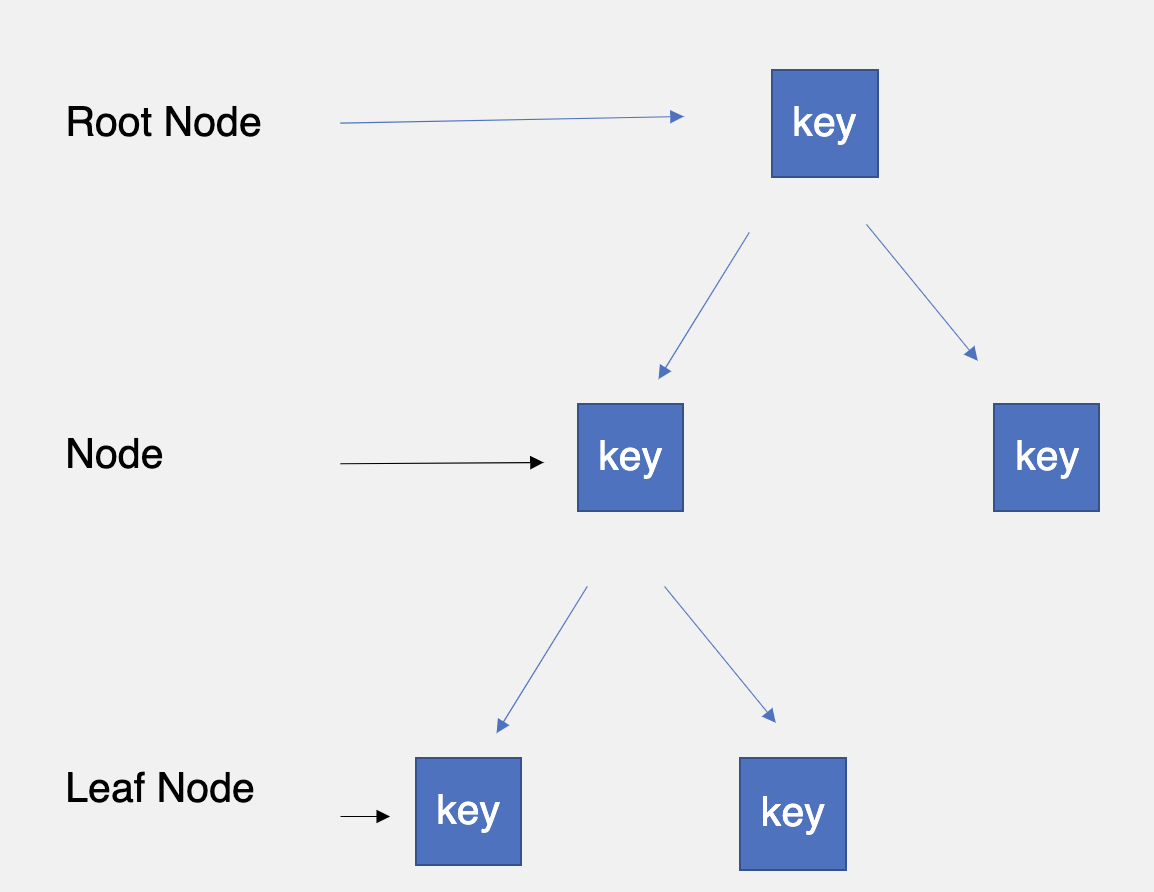
\includegraphics[width=0.6\textwidth]{graphs/KD-Tree.png}
    \caption{KD-Tree}
    \label{fig:KD-Tree}
\end{figure}

\begin{enumerate}
    \item\textbf{{Node}}: Node of a KD-Tree is essentially a 2-dimensional data point. It can be k-dimensional for KD-Tree.
    \item\textbf{{Root Node}}: Root Node is the Node with no parents and has other nodes/leaves as children. Each node can have two child nodes since it is a binary tree. 
    \item\textbf{{Leaf Node}}: Leaves of a tree are the nodes which do not have any child nodes.
    \item\textbf{{Dimensions}}: Every KD-Tree can be structured in such a way that the data points are divided into k-dimensions. Each node is recursively cut into as many dimensions as is mentioned in the dimensions. In our case the data points are 2-dimensional and hence the space is divided in 2-dimensions alternatively until a leaf is reached.\\
\end{enumerate}
    
\begin{algorithm}[H]
    \SetAlgoLined
    \SetKwInOut{Input}{Input}
    \SetKwInOut{Output}{Output}
    \Input{Point list; trainset=[$(x,y);x \in \mathbb{R}^{2};y \in \mathbb{R}$], dimension = 2, $int$ split axis; 0 or 1}
    \Output{KD-Tree}
    \For{$i\gets0$ \KwTo $len(Point list)$}{
    \texttt{$int$ split axis := split axis mod $dim$} // Select the split axis based on depth\\
    \texttt{Sort point list and choose median}\\
    \texttt{Create node at median}\\
    \texttt{node.leftChild := kdtree(points in pointList before median, split axis+1); //SubTree Creation \\ 
    node.rightChild := kdtree(points in pointList after median, split axis+1);}
     \caption{Training Algorithm for KD-Tree}
     \label{Training_KD-Tree}
     }
\end{algorithm}

For constructing the KD-Tree we have following consttraints:


\begin{enumerate}
    \item {As one moves down the tree, one cycles through the axes used to select the splitting planes. For example, in a 2-dimensional plane we split the data on x-axis at the root and then split it on y-axis for it's children. We then split the grandchildren on x-axis again and so on.}
    \item {Points are inserted by selecting the median of the points being put into the subtree, with respect to their coordinates in the axis being used to create the splitting plane. This ensures that the tree is balanced. A balanced tree is the one in which leaf node is approximately the same distance from the root.}\\
\end{enumerate}    
    
In the algorithm above, we first sort all the values obtained in the Point list. We initialise the first split axis to 0 and then toggle between 0 and 1 as we increase the depth. Once the data points are sorted, their median is chosen. For example if we have points sorted as [[3,4],[5,6],[7,8]], we will take the median as [5,6] and assign [3,4] to the left and [7,8] to the right. The reason node.leftChild = [1,2] is because 1 < 5 and node.rightChild = [7,8] is because 7 > 5 i.e., we compare the x-axis of the points to the root when we create the subsequent nodes. This process is then carried out recursively and subtrees are created on the left and right until all the points are added to the tree from the Point list.

\subsubsection{Construction time of 2-dimensional kd-tree:}

The most expensive part of the construction of KD-Tree is sorting the points on both the axis. Instead of working with more complex algorithm to find the median we first presorted the values on x-axis and then on y-axis. Hence the time complexity is $O( n log n)$. Since KD-Tree is A binary tree, and every leaf and internal node uses O(1) storage, the total storage is $O(n)$.


\subsubsection{Introduction to Range Searching}

\begin{figure}[htp]
    \centering
    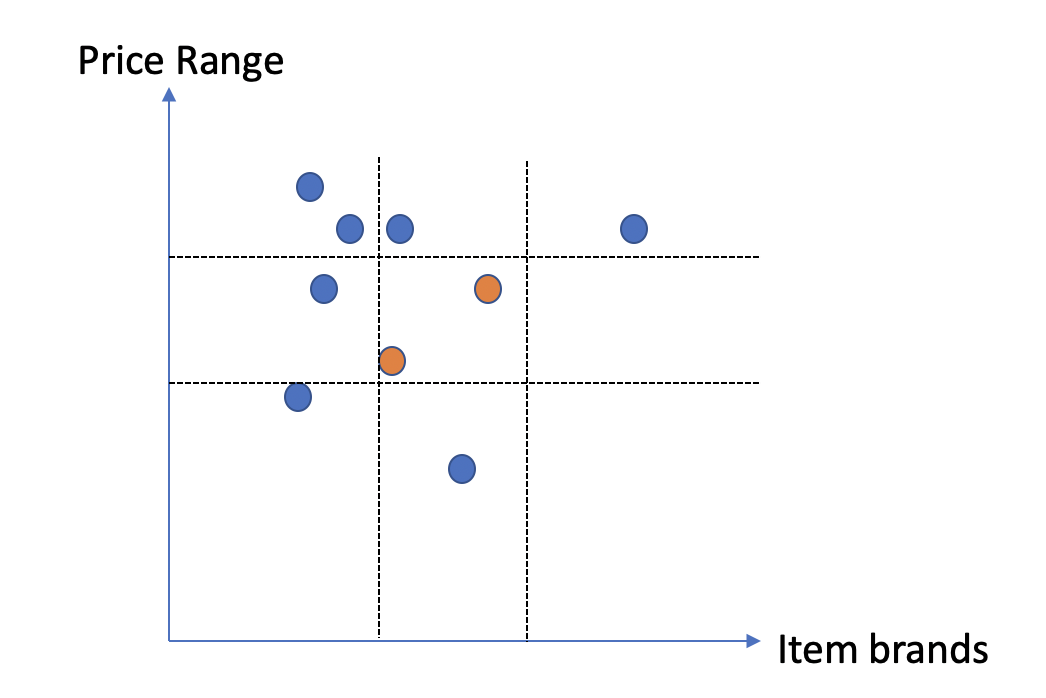
\includegraphics[width=0.6\textwidth]{graphs/Range_Query_Intro.png}
    \caption{KD-Tree Range Query}
    \label{fig:KD_ee_Range_Query_Intro}
\end{figure}

Range searching is basically to search data which lie within a specified range. For example if you have a database where you store data of a number of items and their price ranges. You want to search items from a specific brand and within a specific price range. You can search for this data by specifying these parameters. In our model we can pass the lower bound and upper bound of a rectangle and all the points that lie within those bounds are retrieved in the 2-dimensional plane.


\begin{figure}[htp]
    \centering
    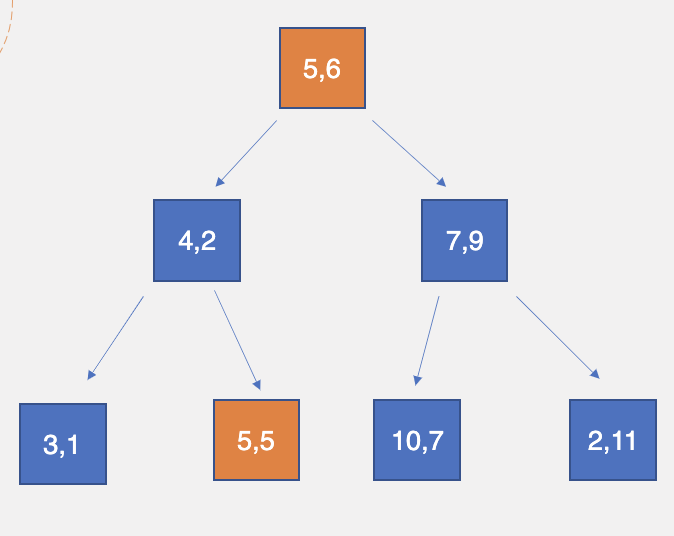
\includegraphics[width=0.6\textwidth]{graphs/Range_Query_Tree.png}
    \caption{KD-Tree for Range Query}
    \label{fig:KD-Tree_for_Range Query}
\end{figure}

\begin{figure}[htp]
    \centering
    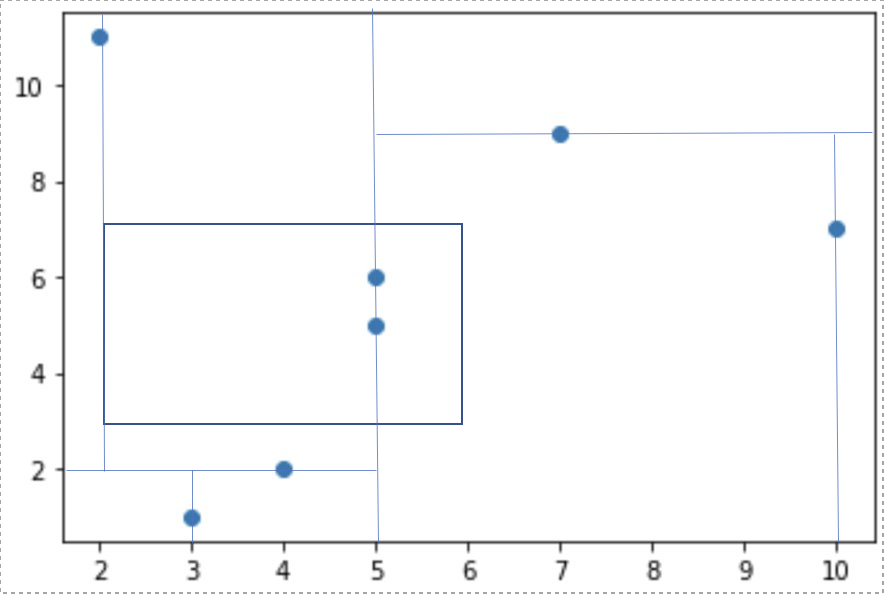
\includegraphics[width=0.6\textwidth]{graphs/Range_Query_plot.png}
    \caption{KD-Tree Range Query Plot on 2-dimentional plane}
    \label{fig:KD_Tree_Range_Query_Plot}
\end{figure}

In our model in range query we first generate lower and upper bound of the rectangle randomly. We then check if the root of the tree lies within the range of the bounds and only then start traversing the tree. For example we have a tree with Point list as 

	$$[(5,6),[4,2],[7,9],[3,1],[5,5],[10,7],[2,11]]$$
	
	and with lower bound = [2,3] and upper bound = [6,7], we will get a tree as is shown in \ref{fig:KD-Tree_for_Range Query}. We can see the points along with the rectangle range plotted in \ref{fig:KD_Tree_Range_Query_Plot}. Points [5,5] and [5,6] are returned in the query since they lie within the rectangle as seen in the plot. First the root point is checked and since the x coordinate and y coordinate both lie within the rectangle bounds i.e., 2 > 5 > 6 and 3 > 6 > 7. It then checks if the x coordinate is lower than or greater than the lower bound x coordinate. Since the value is larger than lower bound x coordinate that is 2 it will then traverse to the left. In the left it has child node as [4,2] however, since the y coordinate doesn't lie in the range of the upper bound this point is not selected. Therefore, it recursively traverses the tree and checks if the point lies within the bound until it reaches a leaf.

\subsubsection{K-nearest neighbour}

K-nearest neighbour as the name suggests is the process to find the k nearest neighbour to the test point that we are looking for. For example in a database if you have coordinates of various famous restaurants stored and you want to query 5 nearest restaurants to your current location then the query should fetch you 5 nearest restaurants depending on your current location on the map. Your current coordinate can be any value and may not be a subset of the data. \\

In our model k-nearest neighbour is calculated based on the euclidean distance of the test data point with respect to the other points. We have also compared the result of our model with standard packages of scipy sklearn to verify the results of the distance calculated and the points returned. Since measuring distance of each point from the test point is computationally very expensive we exploit the tree structure of the KD-Tree to prune the tree and only measure distance with much fewer points and only traverse a subtree if required. \\

\begin{figure}[htp]
    \centering
    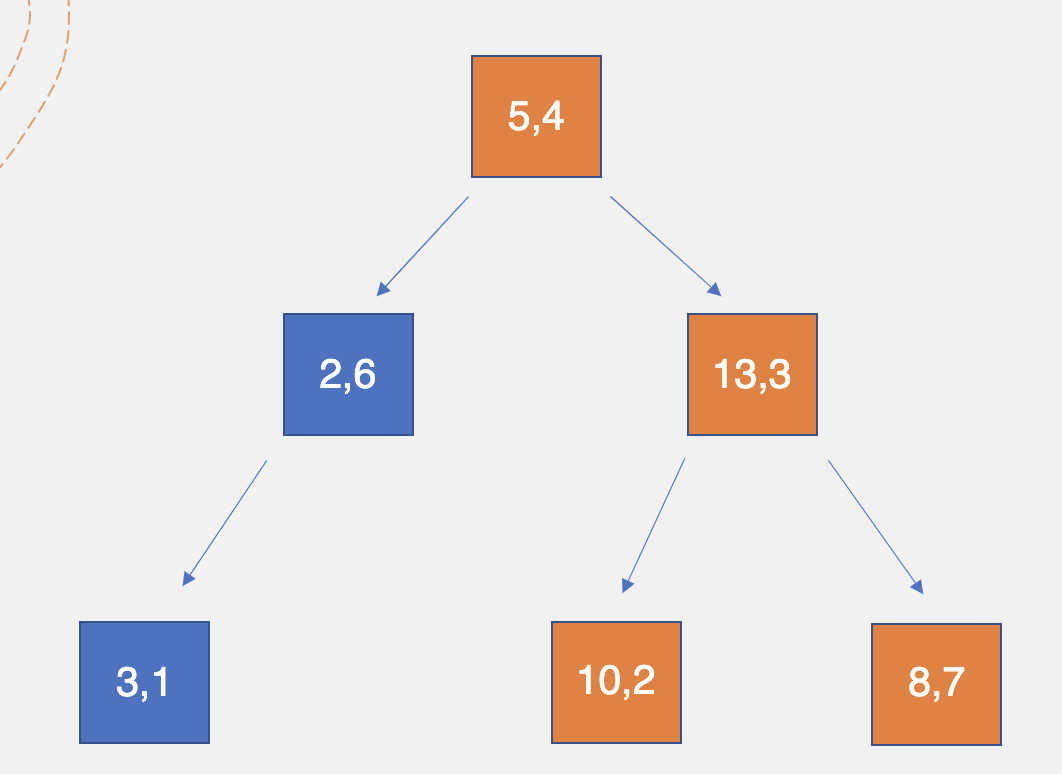
\includegraphics[width=0.6\textwidth]{graphs/KD-Tree_KNN_Tree.png}
    \caption{KD-Tree for KNN Query}
    \label{fig:KD-Tree_for_KNN Query}
\end{figure}

\begin{figure}[htp]
    \centering
    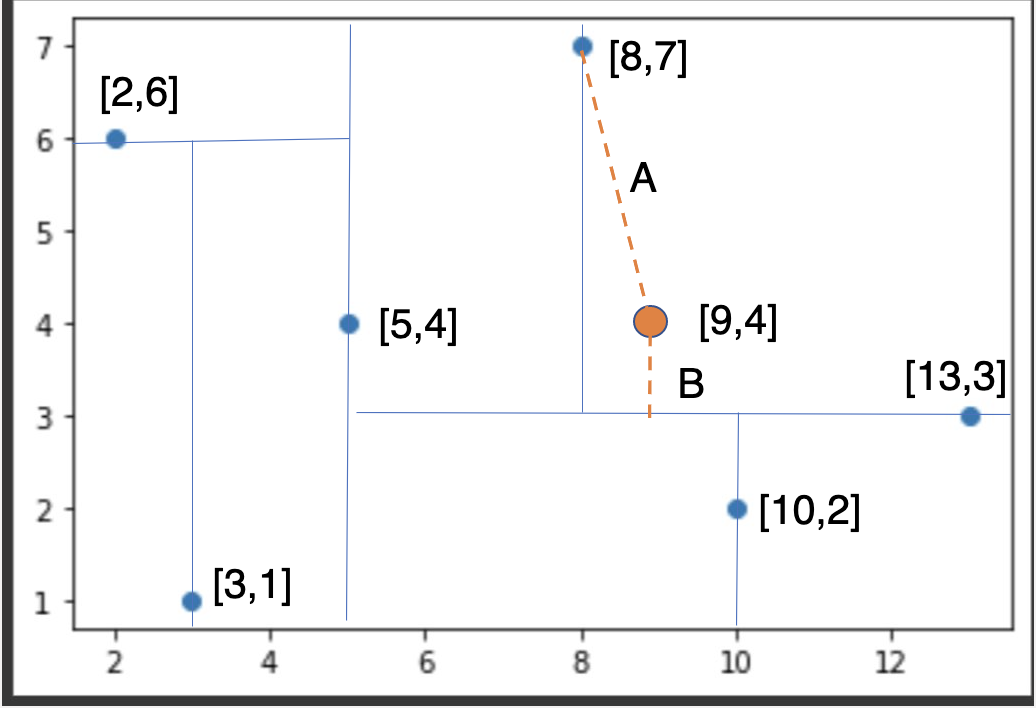
\includegraphics[width=0.6\textwidth]{graphs/KD-Tree_KNN_plot.png}
    \caption{KD-Tree KNN Plot on 2-dimentional plane}
    \label{fig:KD_Tree_KNN_Plot}
\end{figure}


\begin{mscexample}
	For example, we have Point list as $[(5,4),[2,6],[13,3],[8,7],[3,1],[10,2]]$ then we will have a tree structure as shown in \ref{fig:KD-Tree_for_KNN Query} and it's plot on 2-dimensional plane is shown in \ref{fig:KD_Tree_KNN_Plot}. As we can see in \ref{fig:KD_Tree_KNN_Plot} that even though point [8,7] is the leaf we will reach when we traverse the tree to search for point nearest to test point [9,4] it is not infact the nearest point to the test data. In this case if we want to look for 4 nearest neighbour, we first check the square of euclidean distance of [9,4] with the root of the tree i.e., [5,4] which is 16. It then calculates the distance with [2,6] and [13,3] which calculates to 53 and 17 respectively. It then keeps traversing to the right node while calculating distance until it reaches a leaf. After reaching the leaf it then checks the distance with [8,7] with a distance of 10 which is infact smaller than the previous shortest distance of 16 with the root. It adds these points to the list. It then makes a decision weather to go left from [13,3] based on the distance of the test point with leaf [8,7] i.e., A and the perpendicular distance with point [13,3] which is B. Since distance A > B as can be seen in the figure \ref{fig:KD_Tree_KNN_Plot} there is a chance that there could a point in the subtree with a distance smaller than the previous points. In this case it will then check the distance with point [10,2] and the distance is the shortest(best distance) so far of 5. 
\end{mscexample}



\subsubsection{Point Query with Baseline Index Model}

\subsubsection{Overview}

The B-Tree can be regarded as a function $\mathcal{F}$ that maps the key $x$ into its corresponding page index $y$. It is known to us that the pages are allocated in a way that the every $S$ entries are allocated in a page where $S$ is a pre-defined parameter. For example, if we set $S$ to be 10 items per page, then the first page will contain the first 10 keys and their corresponding values. Similarly, the second 10 keys and their corresponding values will be allocated to the second page.

If we know the CDF of $X$ as $F(X\leq x)$ and the total number of entries $N$, then the position of $x$ can be estimated as $p=F(x)*N$ and the page index where it should be allocated to is given by

$$y=\floor{\frac{p}{S}}=\floor{\frac{F(x)*N}{S}}$$  

For example, if the keys are uniformly distributed from $0$ to $1000$, i.e. the CDF of $X$ is defined as $F(X\leq x)=\frac{x}{1000}$ and we set $S=10, N=1001$. Then for any key $x$, we immediately know it will be allocated into $y=\floor{\frac{1000}{10}*\frac{x}{1000}}=\floor{\frac{x}{10}}$. Assume that we have a key $698$, then we can calculate $y=\floor{\frac{698}{10}}=69$. By doing so, the page index is calculated in constant time and space.

In this example, we see that the distribution of $X$ is essential and our goal of learned index in one-dimensional data is to learn such distribution. To do so, we apply two different techniques as the baseline, the polynomial regression and fully connected neural network.

To train such a learned index, we first manually generate the $X$ with respect to a certain distribution. We then save the generated $X$ into a dense array with the length $N$. Then we use the proportional index, i.e. the index of each $x$ divided by $N$ as the expected output $y$.

\subsubsection{Polynomial Regression}
 
The polynomial regression model with degree $m$ can be formalised as 

$$ \hat{y_i}= \beta_0+\beta_1x_i+\beta_2x_i^2+\cdots+\beta_mx_i^m$$ and it can be expressed in a matrix form as below

$$
\begin{bmatrix}
y_1 \\ y_2\\ \vdots \\ y_n 
\end{bmatrix}=\begin{bmatrix}
1 & x_1 & x_1^2 &\cdots & x_1^m \\ 
1 & x_2 & x_2^2 &\cdots & x_2^m \\ 
\vdots \\ 
1 & x_n & x_n^2 &\cdots & x_n^m \\ 
\end{bmatrix}\begin{bmatrix}
\beta_0 \\ \beta_1 \\ \vdots \\ \beta_m 
\end{bmatrix}
$$ which can be written as $Y=\boldsymbol{X}\boldsymbol{\beta}$. 
 
 Our goal is to find $\beta$ such that the sum of squared error, i.e. $\text{S}(\boldsymbol{\beta})=\sum_{i=1}^n(\hat{y}-y)^2$ is minimal. This optimisation problem can be resolved by ordinary least square estimation as shown below.
 
 First we have the error as
 
 \begin{equation}
 \begin{split}
 \text{S}(\boldsymbol{\beta})=||\boldsymbol{y}-\boldsymbol{X} \boldsymbol{\beta}||& =(\boldsymbol{y}-\boldsymbol{X}\boldsymbol{\beta})^T(\boldsymbol{y}-\boldsymbol{X}\boldsymbol{\beta})\\
 	& =\boldsymbol{y}^T\boldsymbol{y}-\boldsymbol{\beta}^T\boldsymbol{X}^T\boldsymbol{y}-\boldsymbol{y}^T\boldsymbol{X}\boldsymbol{\beta}+\boldsymbol{\beta}^T\boldsymbol{X}^T\boldsymbol{X}\boldsymbol{\beta}
\end{split}
 \end{equation}
 
 Here we know that $(\boldsymbol{\beta}^T\boldsymbol{X}^T\boldsymbol{y})^T=\boldsymbol{y}^T\boldsymbol{X}\boldsymbol{\beta}$ is a $1\times 1$ matrix, i.e. a scalar. Hence it is equal to its own transpose. As a result we could simplify the error as
 
 \begin{equation}
 	\begin{split}
 		\text{S}(\boldsymbol{\beta})=\boldsymbol{y}^T\boldsymbol{y}-2\boldsymbol{\beta}^T\boldsymbol{X}^T\boldsymbol{y}+\boldsymbol{\beta}^T\boldsymbol{X}^T\boldsymbol{X}\boldsymbol{\beta}
 	\end{split}
 \end{equation}
 
 In order to find the minimum of $S(\boldsymbol{\beta})$, we differentiate it with respect to $\boldsymbol{\beta}$ as 
 
 \begin{equation}
 	\nabla_{\boldsymbol{\beta}}S=-2\boldsymbol{X}^T\boldsymbol{y}+2(\boldsymbol{X}^T\boldsymbol{X})\boldsymbol{\beta}
 \end{equation}
 
 By let it to be zero, we end up with 
 
 \begin{equation}
 \begin{split}
 	 &	-\boldsymbol{X}^T\boldsymbol{y}+(\boldsymbol{X}^T\boldsymbol{X})\boldsymbol{\beta}=0 \\
 	& \implies \boldsymbol{\beta}= (\boldsymbol{X}^T\boldsymbol{X})^{-1}\boldsymbol{X}^T\boldsymbol{y}
 \end{split}
 \end{equation}
 
\subsubsection{Fully Connected Neural Network}

\subsubsection{Point Query with Recursive Model Index}

%TODO: there should be some graph to demonstrate the last-mile problem.

In our baseline models, it is not very difficult to reduce the mean square error from millions to thousands. However, it is much harder to reduce it from thousands to tens. This is the so called last-mile problem.

In order to solve this problem, recursive model index was proposed \cite{kraska2018case}. The idea is to split the whole set of data into smaller pieces and assign each piece an index model. By doing so, each model is only responsible for a small range of keys. Ideally, in each smaller range, the keys are distributed in a way that is easier to be learned by our index models, such as polynomial model, fully connected model or even traditional B-Tree model.

As shown in Fig. \ref{rmi_structure}. A recursive model can be regarded as a tree structure, which contains a root model that receives the full dataset for training. Then the root model will split the dataset into several parts. Each sub-model will then receive one part of the full dataset. Then we train the sub-models one by one with the partial training dataset. 

\begin{mscexample}
	For example, in the Fig. \ref{rmi_structure}, the full dataset will be split into three parts and each sub-model receives one part. To train this recursive model, we first train the root model with the whole dataset. Then the root model will split the dataset into 3 parts according to the predicted value of each data point in the dataset. Then each sub-model will receive one part and we train the sub-model accordingly.
\end{mscexample}

\begin{figure*}[h]
\centering
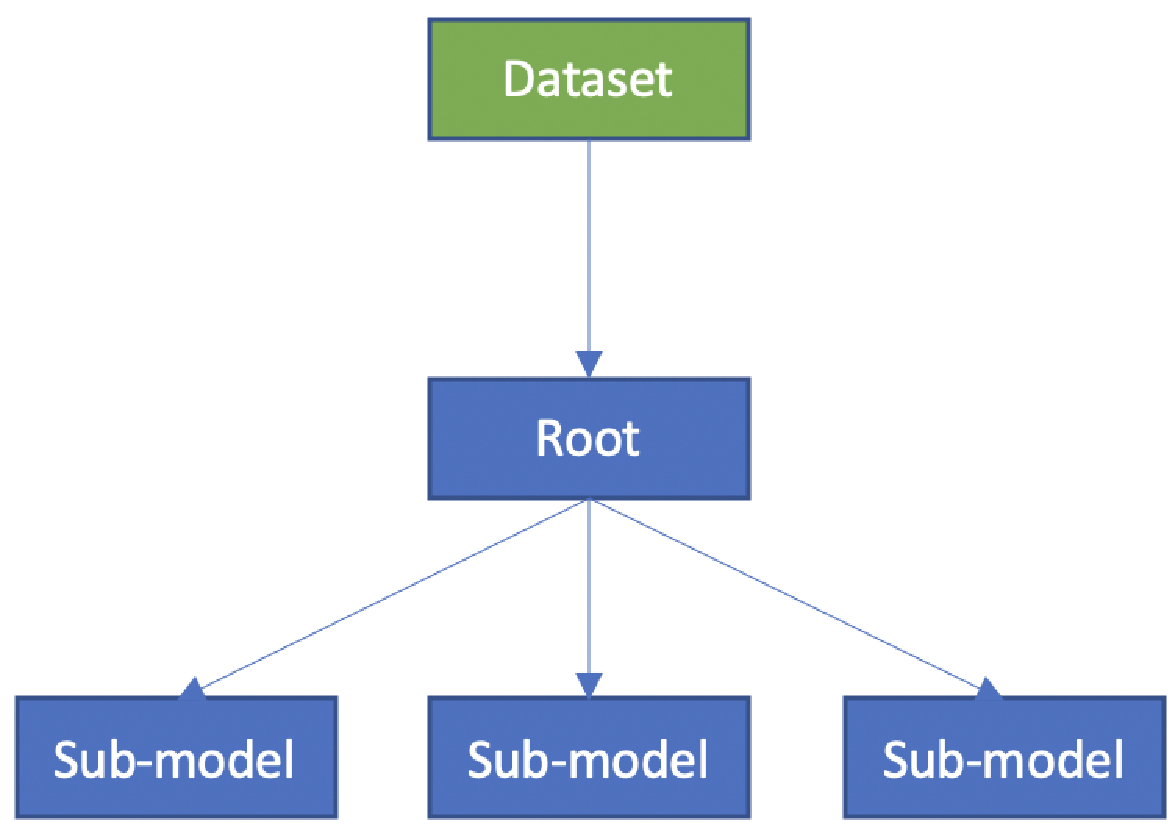
\includegraphics[scale=0.4]{graphs/rmi_demo}
\caption{An example recursive model index with one root model and three leaf model.}
\label{rmi_structure}
\end{figure*}



\subsubsection{Definitions}

Similar to a tree, we define the following terms in a recursive model:

\begin{enumerate}
	\item \textbf{Node Model}. Every node is responsible for making decisions with given input data. In one dimensional case, it can be regarded as a function $f:\mathbb{R}\to\mathbb{R}, x\to y$ where $x$ is the input index and $y$ is the corresponding page block. In principle, each node can be implemented as any machine learning model, from linear regression to neural network, or a traditional tree-based model, such as B-Tree.
	\item \textbf{Internal Node Model}. Internal nodes are all nodes except for leaf nodes and the root node. Every internal node receives a certain part of training data from the full dataset, and train a model on it. 
\end{enumerate}

In the following sections, we will use the notations defined below:
\begin{enumerate}
	\item $N_M^{(i)}$ is the number of models in the $i$th stage.
	%TODO: more notations
	%TODO: modify algorithms accordingly
\end{enumerate}


\subsubsection{Training}

In order to construct a recursive model, we need to have several parameters listed below:
\begin{enumerate}
	\item The training dataset, notated as $(X, Y)$ with entries notated as $(x,y)$.
	\item The number of stages, notated as $N_S$. It is an integer variable.
	\item The number of models at each stage, notated as $N_M$. It is a list of integer variable. $N_M^{(i+1)}$ represents the number of models in the $i$th stage.
\end{enumerate}

The training process of recursive model is an up-bottom process. There will be only one root model that receives the whole training data. After the root model is trained, we iterate over all the training data and predict the page by the root model. After the iteration, we get a new set of pairs $(X, Y_0)$. Then we map $\forall y_0\in Y_0$ into the selected model id in next stage by $\texttt{next}=y_0 * N_M^{(i+1)}/\texttt{max(Y)}$.

\begin{algorithm}[H]
    \SetAlgoLined
    \SetKwInOut{Input}{input}
    \Input{\texttt{num\_of\_stages; num\_of\_models; types\_of\_models; x; y}}
     \texttt{trainset=[[(x,y)]]} \\
     \texttt{stage$\gets 0$} \\
     \While{\texttt{stage} \textless \texttt{num\_of\_stages}}{
      \While{\texttt{model} \textless \texttt{num\_of\_models[stage]}} {
        \texttt{model.train(trainset[stage][model])} \\
        \texttt{models[stage].append(model)}
      }
      \uIf{not last stage} {
        \For{$i\gets0$ \KwTo $len(x)$}{
            	\texttt{model=models[output from previous stage]} \\
            	\texttt{output=model.predict(x[i])} \\
            	\texttt{next=output * num\_of\_models[stage+1]/max\_y} \\
            	\texttt{trainset[stage+1][next].add((x[i],y[i]))}
        }
      }
     }
     \caption{Training of Recursive Model Index}
\end{algorithm}

\subsubsection{Prediction}

\begin{algorithm}[H]
    \SetAlgoLined
    \SetKwInOut{Input}{input}
    \Input{\texttt{x; models; num\_of\_stages; max\_y}}
     \texttt{stage$\gets 0$} \\
 	 \texttt{next\_model$\gets 0$} \\
     \While{\texttt{stage} \textless \texttt{num\_of\_stages}}{
        \texttt{output = model.predict(x)} \\
        \texttt{next\_model=output*len(models[stage+1])/max\_y}\\ 
      \uIf{last stage} {
		\texttt{y = next}
      }
     }
     \caption{Training of Recursive Model Index}
\end{algorithm}

\subsubsection{Polynomial Internal Models}

In the recursive model index, we use internal models to learn the CDF of a part of the full training data. In order to learn the CDF, we need to know or assume the distribution of a specific part of the data. In this report, we support the following distributions.

\begin{table}[h]
  \begin{tabularx}{\textwidth}{@{}XX@{}}
  \toprule
    Linear Regression & $wx+b$ \\
    Quadratic Regression & $ax^2+bx+c$ \\
    B-Tree & N/A \\
    Fully Connected Neural Network & N/A \\
  \bottomrule
  \end{tabularx}
  \end{table}

Here we describe how we fit a polynomial model.

The polynomial regression model with degree $m$ can be formalised as 

$$ \hat{y_i}= \beta_0+\beta_1x_i+\beta_2x_i^2+\cdots+\beta_mx_i^m$$ and it can be expressed in a matrix form as below

$$
\begin{bmatrix}
y_1 \\ y_2\\ \vdots \\ y_n 
\end{bmatrix}=\begin{bmatrix}
1 & x_1 & x_1^2 &\cdots & x_1^m \\ 
1 & x_2 & x_2^2 &\cdots & x_2^m \\ 
\vdots \\ 
1 & x_n & x_n^2 &\cdots & x_n^m \\ 
\end{bmatrix}\begin{bmatrix}
\beta_0 \\ \beta_1 \\ \vdots \\ \beta_m 
\end{bmatrix}
$$ which can be written as $Y=\boldsymbol{X}\boldsymbol{\beta}$. 
 
 Our goal is to find $\beta$ such that the sum of squared error, i.e. $\text{S}(\boldsymbol{\beta})=\sum_{i=1}^n(\hat{y}-y)^2$ is minimal. This optimisation problem can be resolved by ordinary least square estimation as shown below.
 
 First we have the error as
 
 \begin{equation}
 \begin{split}
 \text{S}(\boldsymbol{\beta})=||\boldsymbol{y}-\boldsymbol{X} \boldsymbol{\beta}||& =(\boldsymbol{y}-\boldsymbol{X}\boldsymbol{\beta})^T(\boldsymbol{y}-\boldsymbol{X}\boldsymbol{\beta})\\
 	& =\boldsymbol{y}^T\boldsymbol{y}-\boldsymbol{\beta}^T\boldsymbol{X}^T\boldsymbol{y}-\boldsymbol{y}^T\boldsymbol{X}\boldsymbol{\beta}+\boldsymbol{\beta}^T\boldsymbol{X}^T\boldsymbol{X}\boldsymbol{\beta}
\end{split}
 \end{equation}
 
 Here we know that $(\boldsymbol{\beta}^T\boldsymbol{X}^T\boldsymbol{y})^T=\boldsymbol{y}^T\boldsymbol{X}\boldsymbol{\beta}$ is a $1\times 1$ matrix, i.e. a scalar. Hence it is equal to its own transpose. As a result we could simplify the error as
 
 \begin{equation}
 	\begin{split}
 		\text{S}(\boldsymbol{\beta})=\boldsymbol{y}^T\boldsymbol{y}-2\boldsymbol{\beta}^T\boldsymbol{X}^T\boldsymbol{y}+\boldsymbol{\beta}^T\boldsymbol{X}^T\boldsymbol{X}\boldsymbol{\beta}
 	\end{split}
 \end{equation}
 
 In order to find the minimum of $S(\boldsymbol{\beta})$, we differentiate it with respect to $\boldsymbol{\beta}$ as 
 
 \begin{equation}
 	\nabla_{\boldsymbol{\beta}}S=-2\boldsymbol{X}^T\boldsymbol{y}+2(\boldsymbol{X}^T\boldsymbol{X})\boldsymbol{\beta}
 \end{equation}
 
 By let it to be zero, we end up with 
 
 \begin{equation}
 \begin{split}
 	 &	-\boldsymbol{X}^T\boldsymbol{y}+(\boldsymbol{X}^T\boldsymbol{X})\boldsymbol{\beta}=0 \\
 	& \implies \boldsymbol{\beta}= (\boldsymbol{X}^T\boldsymbol{X})^{-1}\boldsymbol{X}^T\boldsymbol{y}
 \end{split}
 \end{equation}

  

\subsubsection{Point Query with Lisa}

\comm{
\subsubsection{LISA Baseline model Limitation}

Prediction cost in baseline method consists of following two parts.

\begin{enumerate}
	\item Search cost for the cell which contains the key. This cost will be equal to $log_{2}N_{1}$, where $N_{1}$ is the number of cells into which mapped values are divided.
	
	\item Cost associated with sequentially comparing the query point key value against keys inside the cell found in previous search. On average this cost will be equal to $N_{2}\slash2$, where $N_{2}$ is the number of keys in a cell.   
	
If cell size is large, number of cells will be smaller, number of keys per cell will be higher, resulting in higher cost of sequential scan with in the cell. 
\end{enumerate}
Consider the example in figure \ref{fig:BaseLine_Method_Limitation}. Dataset is divided into 3 sections based on the mapped values. Any point or range query in the second triangle(page) will result into a sequential scan through all 9 keys in the cells.

\begin{figure*}[t]
    \centering
    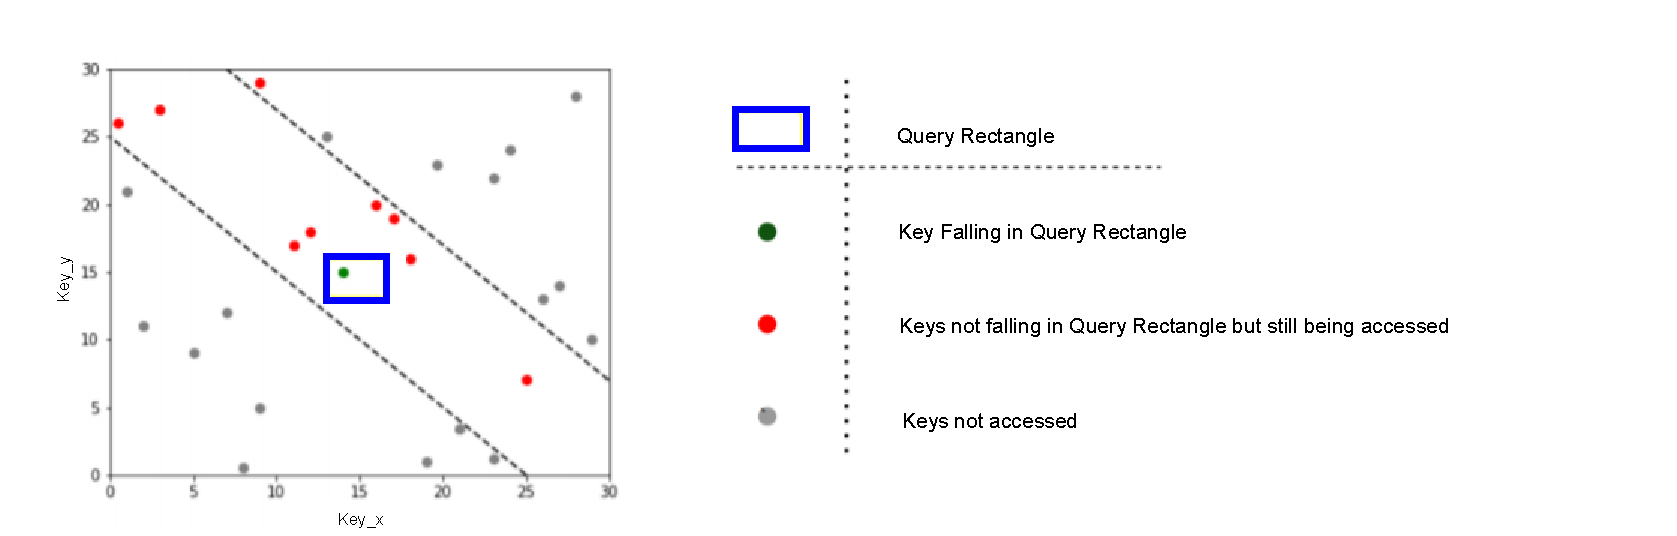
\includegraphics[width=1.3\textwidth]{graphs/Baseline_limitation.pdf}
    \caption{Baseline Method Limitation }
    \label{fig:BaseLine_Method_Limitation}
\end{figure*}
}


\subsubsection {LISA Baseline model search optimization for smaller values of N}
%In lisa baseline model, we need to linearly search for the query key in a cell. 
In case of high dimensional key values, key with in a cell can not be searched with mapped value, as a large number of keys can have the same mapped value. However for the 2 dimensional scenario, we can get considerable savings in search cost by replacing sequential scan based on keys values to binary search based on mapped value. As in the original method, search process  will consist of two parts.
\begin{enumerate}
	\item Find the cell which contains the query key based on mapped value using binary search. 
	\item With in the cell, replace sequential search based on query key value with the  binary search based on query key mapped value. Once mapped value is found, do a lookup in the neighbourhood of the found key based on query key 2 dimensional value. 
\end{enumerate}
As shown in Fig. \ref{fig:LISA_Baseline_Optimization}, we get significant savings in the query time with this approach for smaller values of N. As the value of $N$ increases, number of Keys per cell decreases, and savings in avoiding sequential search gets normalized. 


\begin{figure}
 \centering
     \begin{subfigure}[b]{0.45\textwidth}
         \centering
         \begin{tikzpicture}[font=\small]
	\pgfplotsset{compat=1.10, width=\textwidth, height=\textwidth,every axis
	legend/.append style={
		at={(1,1)},
		anchor=north east}}
	\begin{axis}[
		xmode=log,
		xlabel=$N$,
		ylabel=Average Query Time (ms),
		xtick={10,100,1000,10000},
		legend style={nodes={scale=0.55, transform shape}}
	]
	\addplot[smooth, mark=x, blue]
	coordinates{
		(10, 46.7173)
		(100, 4.8086)
		(1000, 0.7271)
		(10000,0.3301)
		%(100000,0.2381)
	};
	\addplot[smooth,mark=o,red]
  	coordinates{
        (10, 0.2855)
		(100,0.2823)
		(1000, 0.2806)
		(10000,0.2794)
		%(100000,0.2322)
	};
  
    %\legend{LISA Baseline, LISA Baseline Optimized}
	\end{axis}
\end{tikzpicture}
         \caption{Training Size 100K}
         \label{fig:2d_exp4_3_1}
     \end{subfigure}
     \begin{subfigure}[b]{0.45\textwidth}
         \centering
         \begin{tikzpicture}[font=\small]
	\pgfplotsset{compat=1.10, width=\textwidth, height=\textwidth,every axis
	legend/.append style={
		at={(1,1)},
		anchor=north east}}
	\begin{axis}[
		xmode=log,
		xlabel=$N$,
		ylabel=Average Query Time (ms),
		xtick={10,100,1000,10000},
		legend style={nodes={scale=0.75, transform shape}},
		scaled y ticks = base 10:-2,
	]
	\addplot[smooth, mark=x, blue]
	coordinates{
		(10, 347.5613)
		(100, 40.1451)
		(1000, 4.4732)
		(10000,0.6697)
		%(100000,0.2944)
	};
	\addplot[smooth,mark=o,red]
  	coordinates{
        (10, 0.2905)
		(100,0.2858)
		(1000, 0.2844)
		(10000,0.2831)
		%(100000,0.2322)
	};
  
    \legend{LISA Baseline, LISA Baseline Optimized}
	\end{axis}
\end{tikzpicture}
         \caption{Training Size 1M}
         \label{fig:2d_exp4_3_2}
     \end{subfigure}
     \caption{Point query results comparison between LISA Baseline and Optimized Model for different training sizes.}
     \label{fig:LISA_Baseline_Optimization}
\end{figure}


